\section{Literature Review}

\subsection{Detection of Gerrymandering}

- Explain existing research that focuses on whether or not existing maps are gerrymandered

- This is good, but given the move to nonpartisan commissions/collaborations within the state legislatures, it's necessary to have fair methods to generate the districts in the first place. 

- This is why we need.......

\subsection{Automated Redistricting Algorithms}

- Explain purpose of these

- Give some of the first examples

- My research uses three of these, go in depth explaining them. 

\subsubsection{Markov Chain Monte Carlo}

The first automated redistricting algorithm that I'm going to discuss in detail is an implementation of a statistical method known as "Markov Chain Monte Carlo," henceforth MCMC \parencite{fifield2020}.\footnote{I will refer to the \emph{redistricting algorithm} that uses Markov Chain Monte Carlo as "MCMC," rather than the \emph{statistical method} Markov Monte Carlo.} The following overview is meant to provide a high-level understand of how the basic algorithm works. Since the purpose of my research is to compare the \emph{outputs}, that is the redistricting plans, generated by these algorithms, \emph{rather than the algorithms themselves}, a rigorous understanding of the algorithms is not a prerequisite.\footnote{Please see the section "The Proposed Methodology" in the paper for an in-depth, mathematically-rigorous explanation. \parencite[2]{fifield2020}}.

\begin{figure}
    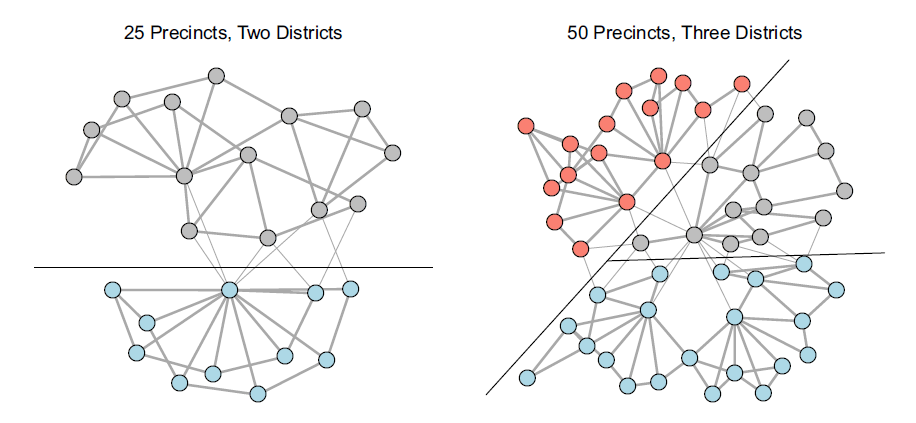
\includegraphics[width=\linewidth]{img/graphcut.png}
    \caption{Representation of redistricting as graph cutting. Every node is a precinct, and nodes that share an edge are known to be adjacent precincts. MCMC "cuts away" edges between nodes until islands of districts are formed. \parencite[3]{fifield2020}}
    \label{fig:graphcut}
\end{figure}

MCMC conceptualizes the problem of redistricting precincts as a graph-cutting problem. For the uninitiated, a graph is a network of different interconnected points, where the points are called "nodes" and the lines connecting them are called "edges" \parencite{fifield2020}. MCMC represents every precinct as a node, and it draws an edge between nodes where the corresponding precincts are adjacent. Since the goal of redistricting is to assign every precinct a district, MCMC imagines that edges between nodes are "cut" until "islands" (known as "sub graphs") are formed, which each is disconnected from the rest. The disconnected "sub graphs" then become the districts. Figure \ref{fig:graphcut} provides a nice visualization of this representation with a sample set of 50 precincts. \parencite{fifield2020}

\begin{figure}
    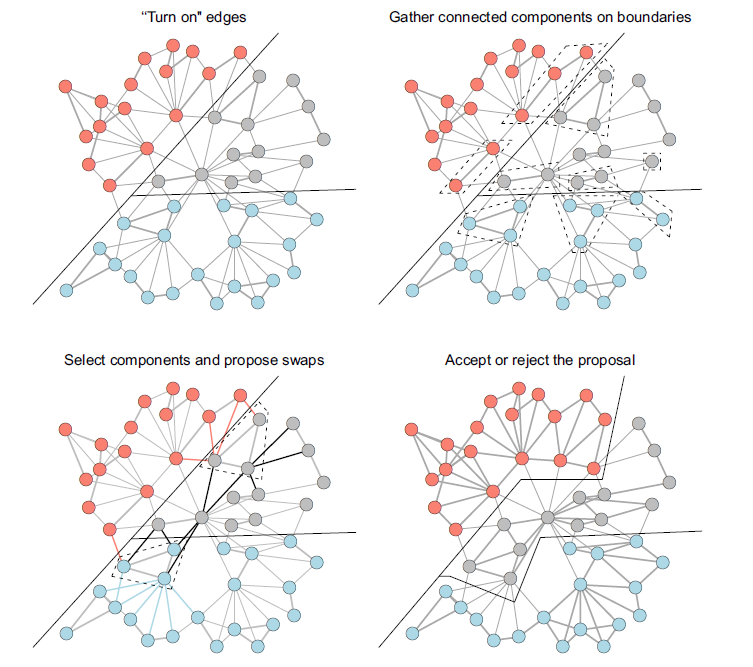
\includegraphics[width=\linewidth]{img/swaps.png}
    \caption{Representation of MCMC algorithm. \parencite[4]{fifield2020}}
    \label{fig:swaps}
\end{figure}

Now that the representation used by MCMC has been established, we can discuss the specifics of the algorithm. Figure \ref{fig:swaps} visualizes the steps in this algorithm. The basic MCMC algorithm begins with a valid redistricting plan, such as the one currently in use, and randomly decides to "turn on" some edges in the graph. Then, the nodes (precincts) that are connected by these "turned on" edges and are located on the boundary of a district are identified. Then, these highlighted graph components are "nominated" for a swap across the district boundary based on some probability, provided that this swap would not break the district into two. Lastly, this new proposed redistricting plan is either accepted or rejected based on some "acceptance probability." This process is repeated as many times as desired. \parencite{fifield2020}.

MCMC in its current form allows for further constraint of this algorithm, particularly with regard to the relative population size and compactness of each district. \parencite[6]{fifield2020} The explanation of thsi algorithm is beyond the scope of this paper. 

\subsubsection{Sequential Monte Carlo}

\subsubsection{Compact Random Seed Growth}

The final automated redistricting algorithm that I'm comparing is called Compact Random Seed Growth, henceforth referred to as "CRSG" and was proposed by \textcite{chen2013}. Its objective is to generate a set of districts that fall within a certain population constraint and are reasonably compact using only the geography and total population of each precinct \parencite{chen2013}. The following is a high-level explanation of the algorithm.\footnote{For more details, please refer to \textcite[249-50]{chen2013}.} 

CRSG begins with declaring that every precinct is it's own district. A random precinct is then chosen, and then its geographically-closest\footnote{The geographically-closest precinct is the neighboring precinct with the smallest distance from its centroid to the seed precinct's centroid} neighboor is mergered with it, creating one fewer district. This process is repeated until you arrive at the desired number of districts. \parencite[249-50]{chen2013}

After this procedure, the districts are somewhat compact due to the geographic proximity requirement, but there is no guarantee that the districts are within the required population percentage of each other. 

To satisfy the population parity requirements, CRSG does the following. First, it identifies the two adjacent districts that have the greatest difference in total population. Then the precinct in the more-populous district that is furthest from the center of said district is reassigned to the less-populous district.\footnote{Provided that this reassignment doesn't break either district into parts.} This process is repeated until all of the districts are within some desired percentage of the mean district population.\textcite[249-50]{chen2013}.

One run of CRSG will produce one set of districts, but separate runs of CRSG with the same input data may produce slightly different districts given the random choice of districts to merge in the first pass of the algorithm. 



\subsection{Empirical Validation}

- Usually small-scale validation within the papers that propose these Algorithms

- Needed to see how well the algorithms scale

- For a commission, it's helpful to be able to compare the results of several different leading algorithms. 

\subsection{Evaluation of Redistricting Plans}

\textcite{katz2020} brings mathematical rigor to the various proposed metrics for measuring partisan symmetry. 

\subsubsection{Partisan Symmetry}

A legislative is said to have partisan symmetry if both parties can receive $m$ proportion of the overall votes and therefore have $n$ proportion of the seats in the legislative body.An example would be that if Republicans win 60\% of the votes but control 65\% of the seats, then in a symmetrical system, Democrats should also be able to control 65\% of the seats by winning 60\% of the votes. \textcite{katz2020}

\begin{figure}
    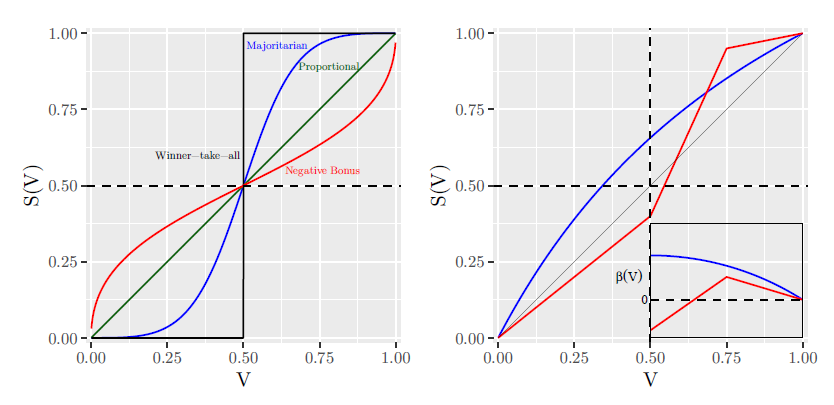
\includegraphics[width=\linewidth]{img/seatsvotes.png}
    \caption{Types of Seats-Votes Curves. Left panel: Symmetric (fair) curves with differing
    levels of electoral responsiveness. Right panel: Asymmetric (biased) curves, including
    one consistently biased toward the Democrats (blue) and one with biases favoring different
    parties depending on V (red); the inset graph is for (V ) for V 2 [0:5; 1] with the vertical
    axis scaled to be the same as the main plot, and lines color coded to the seats-votes curves. \parencite[175]{katz2020}}
    \label{fig:seatsvotes1}
\end{figure}

Partisan symmetry is usually observed by plotting a "seats-votes curve." This plot has $V$, the proportion of the overall votes won by the party, on the x-axis, and $S(V)$, the proportion of the seats won by the party, on the y-axis. Figure \ref{fig:seatsvotes1} \parencite[175]{katz2020} illustrates several hypothetical seats-votes curves.

Naturally, it's very rare to observe the necessary electoral outcomes under the same electoral system in order to determine partisan symmetry. (ie., it's very rare for two parties to tie one year, have one win 51\% of the total votes the next year, and then win 49\% of the votes the following year.)

In practice, one can estimate a seats-votes curve using the principle of uniform partisan swing.

\subsubsection{Uniform Partisan Swing}

Uniform partisan swing is the principle that when the overall vote share $V$ changes by some amount $dV$ between different elections under the same electoral system, the vote share at the district level also usually changes by the same $dV$. \textcite{katz2020} Empirically verified this to be true in 646 different elections. 

Thus, given a list of vote proportions per district ${v_1, v_2, v_3, ...}$ from one election, one can adjust each vote proportion by an arbitrarily small $dV$ until the seats share $S(V)$ is covered from 0 to 1. \parencite{katz2020}.

An example of such a curve is shown in Figure \ref{fig:seatsvotesups1}

\begin{figure}
    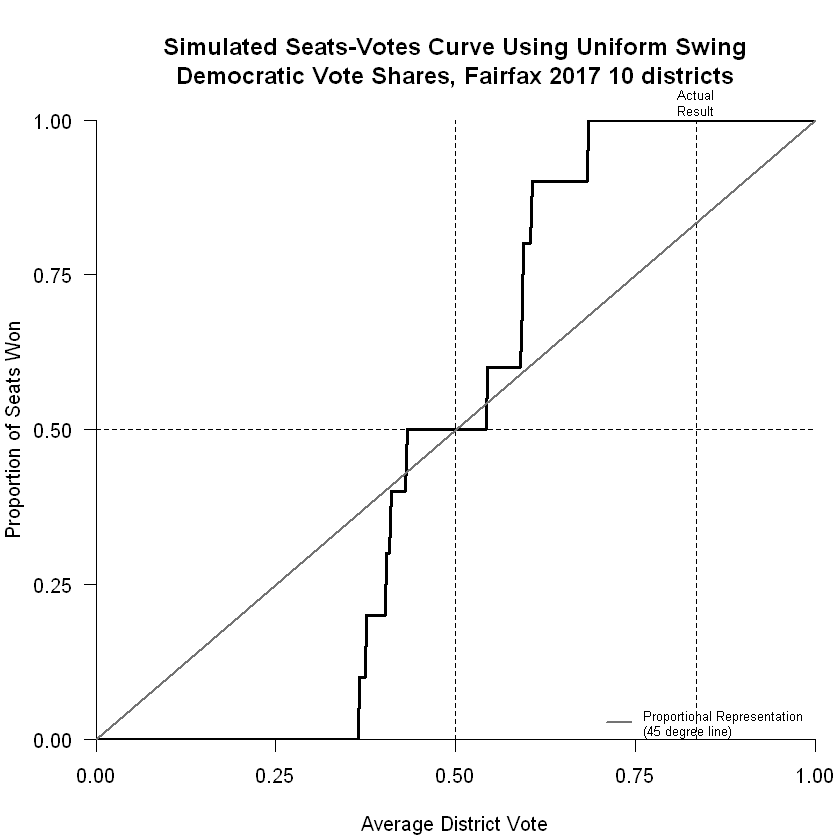
\includegraphics[width=0.5\linewidth]{img/seatsvotesups.png}
    \caption{Sample seats-votes curve generated using uniform partisan swing. Ignore title. \parencite[175]{katz2020}}
    \label{fig:seatsvotesups1}
\end{figure}

